\chapter{O Projeto} \label{int}

O objetivo principal deste projeto é o estudo do desempenho de vários cenários de redes sem fios
para o qual se utiliza técnicas de simulação de eventos discretos. Foram realizados testes para 4 cenários diferentes,para analisar as várias caracteristicas do Wi-Fi e
para isso recorremos ao simulador de rede "ns-3". Todas as simulações apresentadas foram realizadas com um tempo de simulação de 60 segundos.




\section{First Study-Throughput vs Distance} \label{ex1}

    O principal objetivo desta primeira experiência é observar a influencia que a distancia possui sobre a \textit{performance} do \textit{throughput}. Para isso, foram simulados
uma estação (STA) e um ponto de acesso (AP), sendo assim criado um fluxo TCP desde STA para o AP, realizando o envio de um ficheiro grande.
Foram realizadas 16 simulações, entre os 1m e 1500m com um intervalo de 100m entre elas. Conseguimos ver que entre os 1m e 100m a diferença é praticamente nula , 
confirmando que para distâncias curtas o \textit{throughput} é muito semelhante.

\begin{figure}[H]
    \centering
    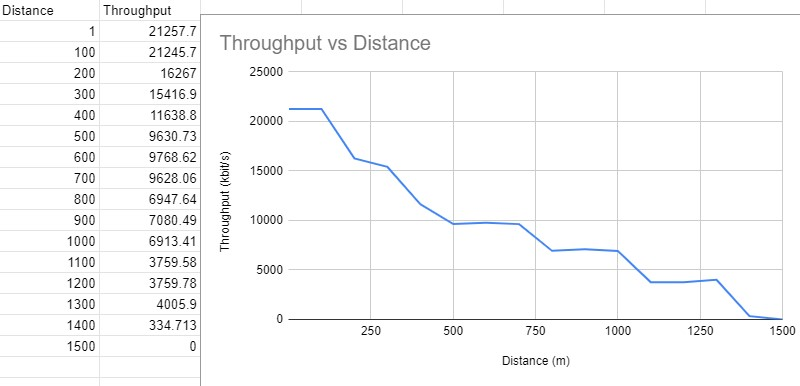
\includegraphics[width=.8\linewidth]{figs/fig1.jpg}
    \caption{Gráfico de Throughput vs Distância}
    \label{fig:1}
\end{figure}

Tal como era esperado de antemão , conforme se aumenta a distância entre a STA e o AP existe uma diminuição de \textit{throughput}, sendo necesário mais tempo para transferir a mesma quantidade
de pacotes, resultado numa pior conexão entre os dois pontos. Verifica-se a existência de alguns "planaltos" em termos de \textit{throughput} como por exemplo entre os 500m e 700m
onde este se mantém em volta dos mesmos valores. Entre os 1300m e 1400m verifica-se uma acentuada redução de \textit{throughput} e nos 100m seguintes a conexão torna-se mesmo nula.


\section{Second Study-Throughput vs Number of STA's} \label{ex2}
    Para a segunda experiência, o objetivo era perceber qual seria o efeito de n STAs a gerar
fluxos TCP para o AP no \textit{throughput}. Foram realizadas 15 simulações partindo de apenas uma STA,
sendo as seguintes adicionadas em torno do AP criando um circulo em torno deste. Recorrendo ao \textit{flowmonitor},
retiramos os valores de \textit{throughput} de cada uma das STAs em direção ao AP.


\begin{figure}[H]
    \centering
    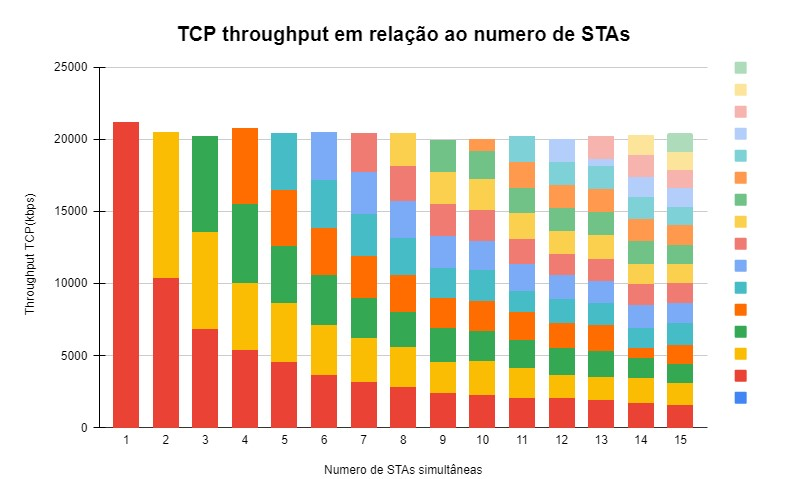
\includegraphics[width=.8\linewidth]{figs/fig2.jpg}
    \caption{\textit{throughput} vs Número de STAs}
    \label{fig:2}
\end{figure}

Analisando o gráfico , conseguimos facilmente retirar que à medida que aumentamos o numero de STAs, a largura de banda de cada é, em média,
distribuida de igual forma por cada uma delas. Isto deriva do facto de o Wi-Fi utilizar o protocolo CSMA/CA , onde o \textit{carrier sense} tenta 
evitar colisões e tornar o acesso ao meio igualmente justo para todos os nós transmissores. No entanto , não é perfeito. Para n=14 , é possivel constatar
que a STA representada pela cor laranja obtem uma quota inferior às restantes.

\begin{figure}[H]
    \centering
    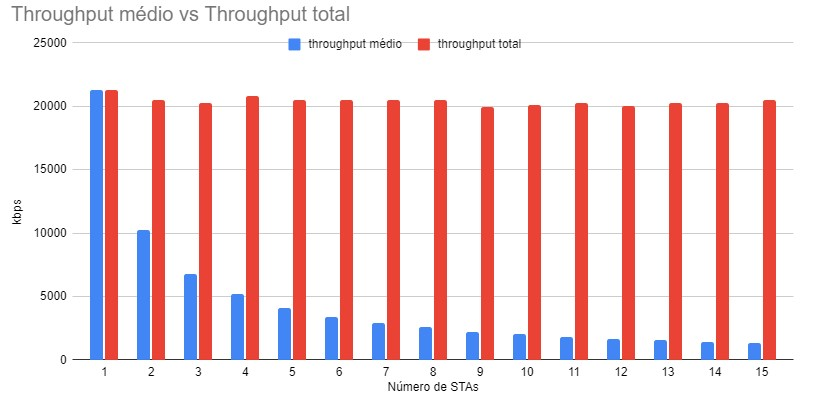
\includegraphics[width=.8\linewidth]{figs/fig3.jpg}
    \caption{Throughput médio vs Throughput total}
    \label{fig:3}
\end{figure}
Assim , e como podemos ver na figura 1.3, o \textit{throughput} médio de cada STA diminui à medida que aumentamos "n" mas o \textit{throughput} total mantem-se 
em torno dos mesmos valores.






\section{Third Study-TCP Throughput vs UDP bitrate} \label{ex3}
    Para a terceira experiência, o estudo consiste em perceber as alterações causadas pela incrementação de tráfico UDP numa 
situação onde existe um AP e duas STA de tráfico UDP e TCP, respetivamente.


\begin{figure}[H]
    \centering
    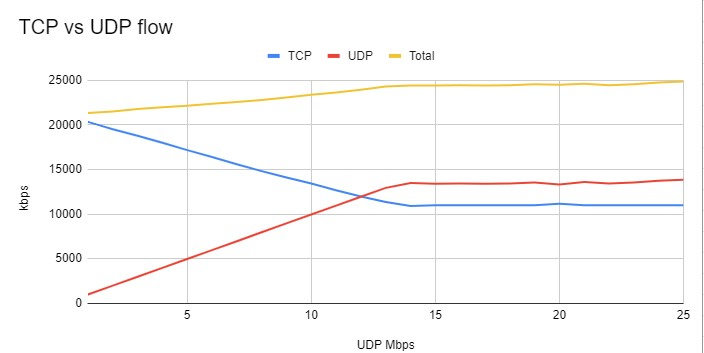
\includegraphics[width=.9\linewidth]{figs/fig4.jpg}
    \caption{trust me dude}
    \label{fig:4}
\end{figure}

O gráfico obtido confirma o que apresentamos anteriormente. À medida que fomos aumentando o fluxo UDP , o fluxo TCP desceu
de forma linear acompanhando em sentido inverso a subida do fluxo UDP.
O protocolo UDP não possui qualquer tipo de controlo de fluxo, fazendo com que este tente sempre usar o máximo fluxo possível que lhe esteja atribuido.
Por outro lado , o TCP utiliza a banda restante entre o máximo possivel e a utilizada pelo fluxo UDP.

Em relação à perda de pacotes , o protocolo TCP possui uma vantagem pelo facto de se adaptar ao \textit{throughput} disponivel
e de efetuar a retransmissão de pacotes, resolvendo este problema. Do lado oposto , o  UDP envia os pacotes sem possuir um
protocolo do tipo "\textit{handshake}" e sem uma ordem particular. Assim , com o aumento do tráfego no meio o numero de pacotes
perdidos era aumentar.


\begin{figure}[H]
    \centering
    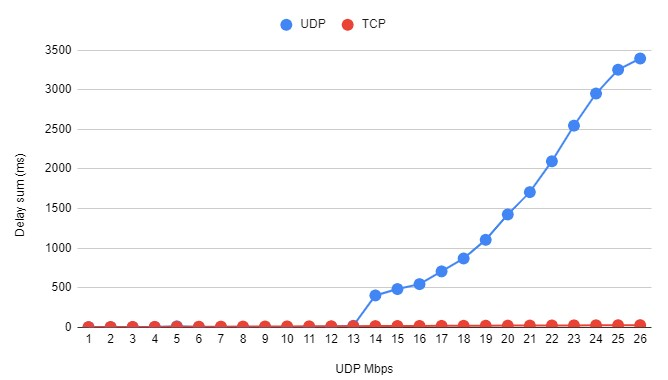
\includegraphics[width=.9\linewidth]{figs/fig6.jpg}
    \caption{Evolução do \textit{delay sum} com aumento do tráfico UDP}
    \label{fig:5}
\end{figure}

Por fim , em relação ao atraso médio dos pacotes conseguimos destacar que existe um grande aumento de atraso dos pacotes para o protocolo
UDP apartir 13-14 mbps, que representa o ponto onde o congestionamento do canal atinge o nivel máximo. Vemos também que
para baixos \textit{bitrates} de UDP, o delay é baixo nos 2 protocolos, sendo o UDP ainda mais baixo. Porém , após os 13 mbps, apesar de um 
grande aumento no \textit{bitrate} do UDP , o protocolo TCP consegue controlar o problema e regista apenas um pequeno aumento, sendo até dificil de visualizar
no gráfico.

%\clearpage

\section{Fourth Study-Throughput vs Distance with relay} \label{ex4}
    Na quarta e ultima experiência, o objetivo é mais uma vez perceber a relação entre o \textit{throughput} e a distância , mas desta vez com uma diferença:
    a utilização de um nó de retransmissão (\textit{relay node}) que se encontra precisamente a meio entre a STA e o AP.
    A utilização de um nó de retransmissão tem como resultado expectável o aumento da distância à qual se consegue manter as comunicações, que na primeira experiência não ultrapassou
    os 1500m. No entanto, as comunicações entre os pontos mais próximos serão prejudicadas em termos de \textit{throughput} uma vez que o mecanismo CSMA/CA irá dividir a capacidade total 
    pelos dois nós, fazendo com que metade da capacidade total seja usada pelo nó de retransmissão mesmo quando este não fosse
    necessário.

    As simulações foram feitas usando incrementos de 100m entre elas tal como na primeira experiência, desde 1m até 3000m.



\begin{figure}[H]
    \centering
    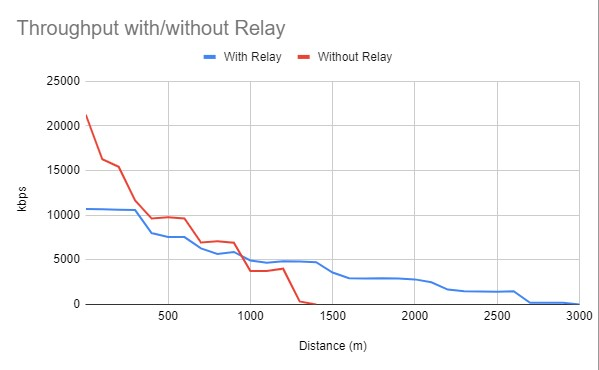
\includegraphics[width=.9\linewidth]{figs/fig5.jpg}
    \caption{}
    \label{fig:5}
\end{figure}

O gráfico a que chegamos corrobora o que foi dito anteriormente. O nó de retransmissão de facto aumenta para cerca do dobro
a distância máxima à qual se consegue manter uma ligação, até um maximo de aproximadamente 3000m . Por outro lado, para transmissões até cerca de 1000m
a utilização do nó de retransmissão é prejudicial pois o \textit{throughput} é inferior ao da transmissão direta até aos 1000m, ponto a partir do qual apesar de ser
possivel uma conexão direta , é mais vantajosa a utilização do \textit{relay}.

Resumindo, a utilização de um nó de  \textit{relay} deve ser reservada para situações com grandes distâncias entre pontos e evitada para situações de curta distância 
uma vez que apenas limita o \textit{throughput} máximo.



